
\documentclass[12pt]{article}

\usepackage{times,fullpage,xspace,fancyhdr}
\usepackage[pdftex]{graphicx}
\usepackage[pdftex,
            a4paper,
            colorlinks=true,
            urlcolor=black,
            linkcolor=black,
            citecolor=black,
            %pagebackref,
            %backref,
            bookmarksopen=false,
            bookmarksnumbered=true,
            pdfstartview=FitH]{hyperref}

\usepackage{epsfig}
\pdfcompresslevel=9
\newcommand{\leaguename}{RoboCup Standard Platform League (Nao) }
\hypersetup{
 pdftitle={\leaguename Rule Book},
 pdfauthor={Technical Committee},
}
\usepackage[latin1]{inputenc}
\usepackage{amsmath}

\newcommand{\ie}{\mbox{i.\,e.}\xspace}
\newcommand{\eg}{\mbox{e.\,g.}\xspace}
\newcommand{\cf}{\mbox{cf.}\xspace}
\newcommand{\comment}[1]{\marginpar{\pdfannot width 4in height .5in depth 8pt {/Subtype /Text /Contents (#1)}}}
\newcommand{\inparagraph}[1]{\paragraph{#1\hspace{-1em} }}

\title{\leaguename Rule Book}
\author{RoboCup Technical Committee}
\date{(2009 rules, as of \today)}

\setlength{\parindent}{0pt}
\setlength{\parskip}{12pt plus 6pt minus 3 pt}
\setcounter{tocdepth}{1}
\widowpenalty=10000
\clubpenalty=10000

\pagestyle{fancy}
\lhead{}
\chead{}
\rhead{}
\lfoot{}
\cfoot{}
\rfoot{}

\renewcommand{\headrulewidth}{0.4pt}
\renewcommand{\footrulewidth}{0.4pt}

\newcommand{\TotalWidth}{{5.4m }}
\newcommand{\TotalLength}{{7.4m }}
\newcommand{\KickOffAutoTime}{{45 seconds }}

\begin{document}

\maketitle

\vfill

\tableofcontents
\setcounter{tocdepth}{3}

\thispagestyle{fancy}

\clearpage

\cfoot{\thepage}
\setcounter{page}{1}

\section{Setup of the Environment}

\subsection{Field Construction}

The soccer field is built on a total carpet area of length \TotalLength  and width \TotalWidth. The dimensions of the soccer field are shown in Figure~\ref{fig:field_dim}. The construction of the goals is depicted in Figure \ref{fig:goal_dimensions}.

\begin{figure}[b!]
\centerline{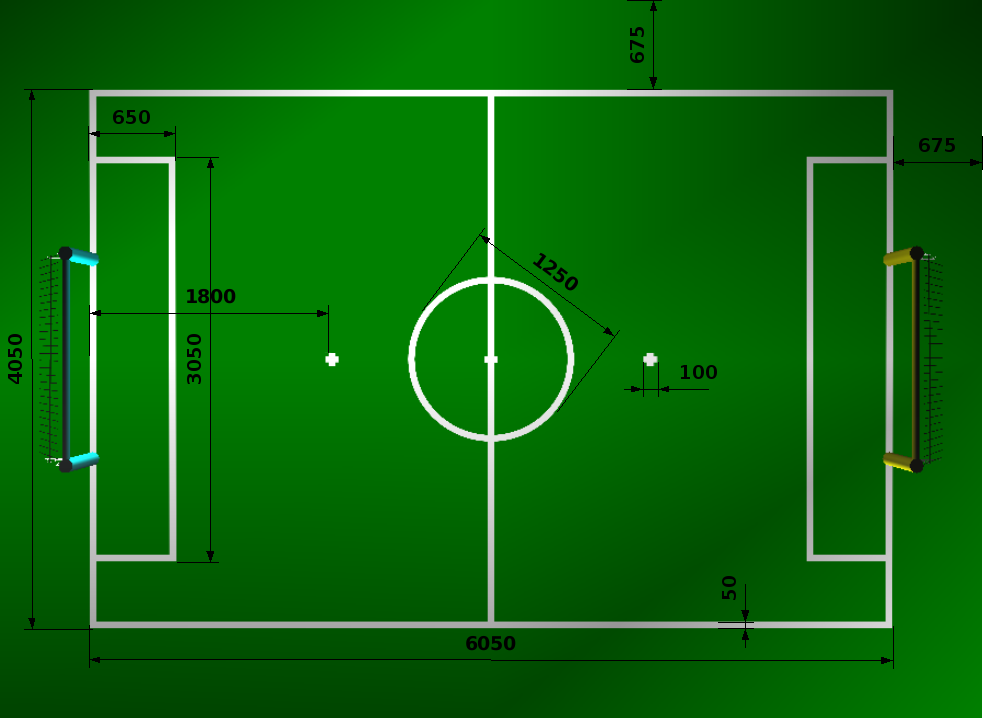
\includegraphics[width=\columnwidth]{figs/fieldDimensions2009.png}}
\caption{Scale diagram of entire field (dimensions in mm).} \label{fig:field_dim}
\end{figure}

%% TAKEN OUT TEMPORARILY...

%\begin{figure}[b!]
%\centerline{\includegraphics[width=0.9\columnwidth]{figs/Field-2d}}
%\caption{Diagram of field not to scale (dimensions in mm).} \label{fig:field_dim2D}
%\end{figure}

%% TAKEN OUT TEMPORARILY...


%\begin{figure}[htp]
%\begin{center}
%    \leavevmode
%    \epsfig{figure=figs/aboveNew.pdf,width=25mm}
%    \epsfig{figure=figs/sideNew.pdf,width=25mm}
%    \epsfig{figure=figs/diagNew.pdf,width=50mm}
%    \caption{Above,side and diagonal views of the new goal.}
%    \label{fig:newgoals}
%\end{center}
%end{figure}


\begin{figure}[htp]
\begin{center}
    \leavevmode
    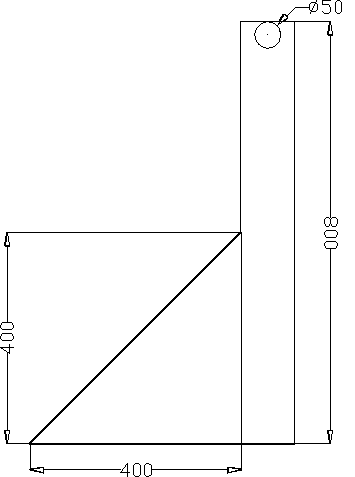
\includegraphics[width=0.4\columnwidth]{figs/goal_with_dims_left.png}\\
    \vspace{10pt}
    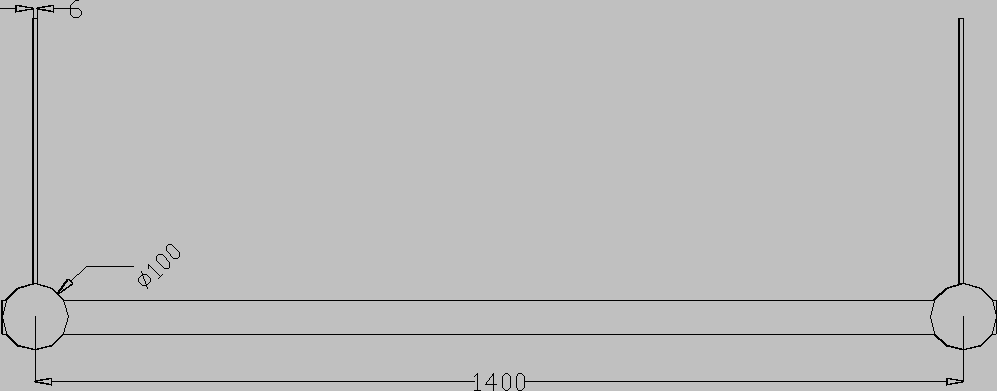
\includegraphics[width=0.8\columnwidth]{figs/goal_with_dims_top.png}
    \caption{Dimensions of the goal, viewed from above and from the side}
    \label{fig:goal_dimensions}
\end{center}
\end{figure}

\subsection{Lines}\label{sec:field_lines}

All robot-visible lines on the soccer field (side lines, end
lines, halfway line, centre circle, corner arcs and the lines surrounding the
penalty areas) are 50~mm in width. The centre circle has an outside diameter of 1250~mm.

%The throw-in lines and corner kick points are not robot visible. The throw-in lines will be marked on the field using a
%thin black or dotted line. The two throw in lines will each be 4m long; parallel to the side lines; and 400mm in from the outside of the side lines.

%RHM 27/4/09
\emph{There are two other sets of unmarked field positions.
(i) throw-in locations (see Section \ref{sec:throw_in}): these are two lines, each 4m long, centered lengthwise with respect to the field, and parallel and 400mm from the to the outside lines.
(ii) corner kick locations (see Section \ref{sec:throw_in}: 
The four corner kick points (not shown in the diagram) are located 400mm towards the centreline from each penalty box corner.
}
\subsection{Field Colors}

The colors of the soccer field are shown in
Figure~\ref{fig:field_color}. All items on the RoboCup field are
color-coded:

\begin{itemize}
\item The field (carpet) itself is green.
\item The lines on the field are white.
\item The red team defends the yellow goal.
\item The blue team defends the sky-blue goal.
\item Goals~(\cf Figure~\ref{fig:goal_colors}). The posts and top cross
  bar are either yellow or sky-blue. The support triangles on back of the posts and the net are white.
\end{itemize}

\begin{figure}[htp]
\begin{center}
    \leavevmode
    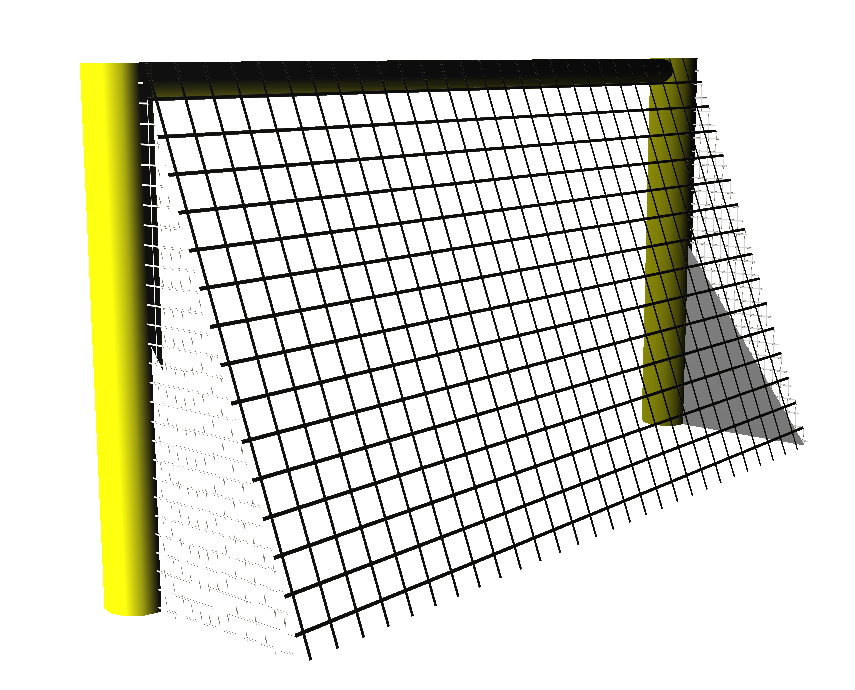
\includegraphics[width=0.45\columnwidth]{figs/GoalBack}
    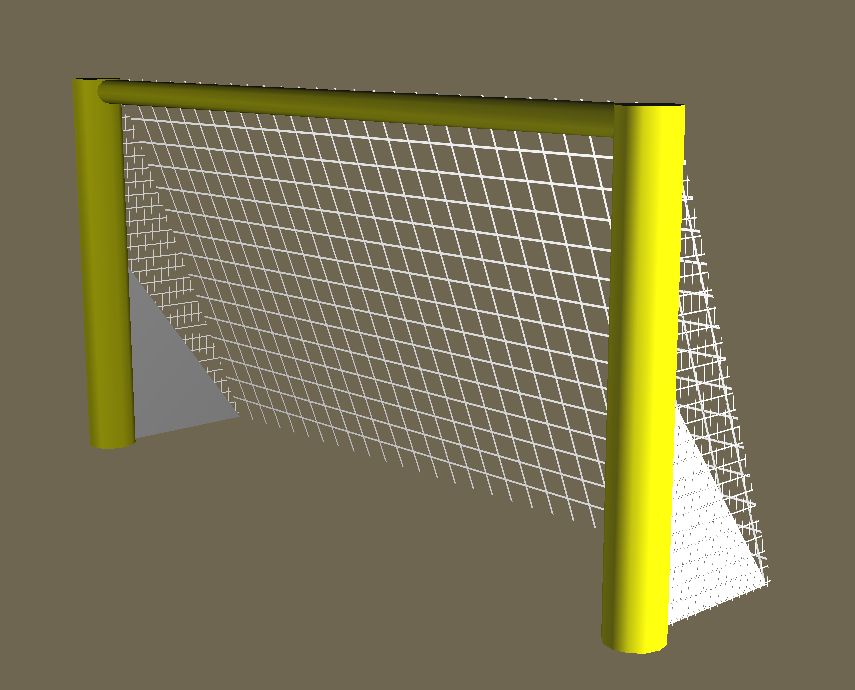
\includegraphics[width=0.45\columnwidth]{figs/GoalFront}
    \caption{Appearance of the yellow goal. Notice that the support triangles are white}
    \label{fig:goal_colors}
\end{center}
\end{figure}

\begin{figure}[t]
\centerline{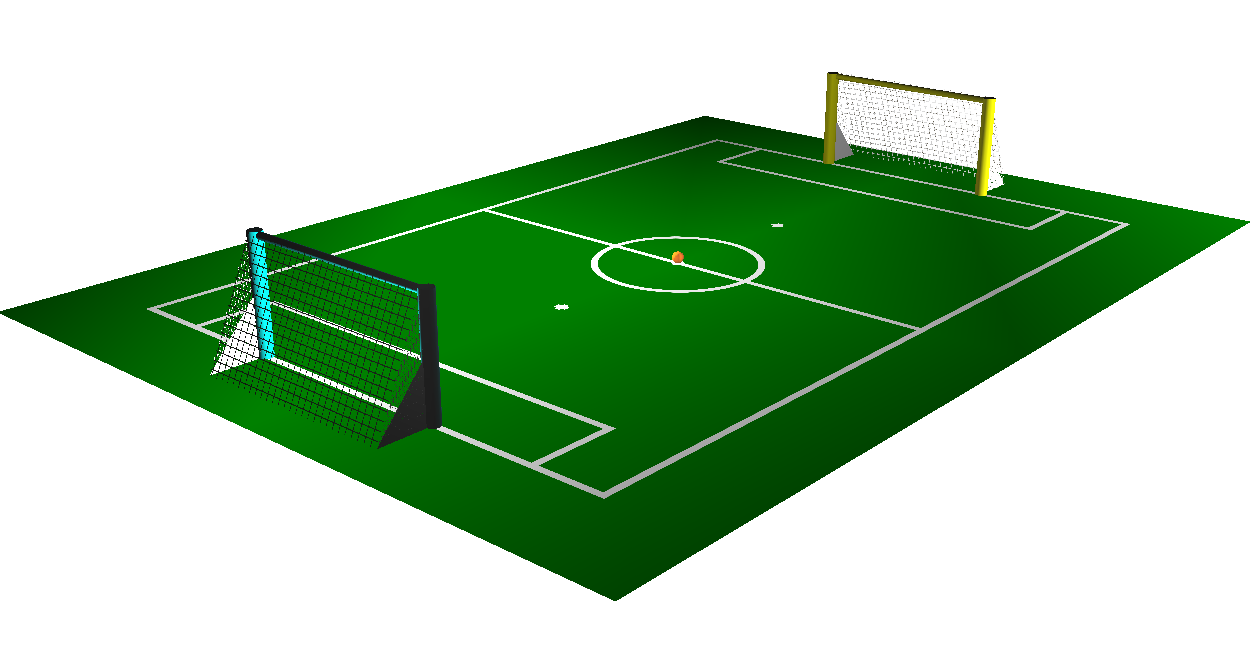
\includegraphics[width=\columnwidth]{figs/Nao2009Field-View.png}}
\caption{Field colors and layout.}
\label{fig:field_color}
\end{figure}


\subsection{Lighting Conditions}
The lighting conditions depend on the actual competition site.
Lighting temperature may differ significantly from previous years, as
only ceiling lights may be used. The lighting level is likely to be lower than that used in previous years.

\section{Robot Players}

\subsection{Hardware}

All teams must use Nao humanoid robot manufactured by Aldebaran Robotics. Absolutely no
modifications or additions to the robot hardware are allowed. No
additional hardware is permitted including off-board sensing or
processing systems. Additional sensors besides those originally
installed on the robots are likewise not allowed. The only
exceptions are:

\begin{itemize}
\item Attaching the official red or blue plastic team markers to the robots.
\item Attaching the jersey numbers provided by the league to the robots.
\item Adding black and white sponsor or team logos to the upper legs of the
robots. These logos must be at least 50\% white by area.
\item Setting the passive wrist joints to a fixed position either with glue or a transparent duct tape.
\item Use of alternate memory sticks in replacement of the Aldebaran supplied memory sticks.
\end{itemize}

A computer will be provided by the event organizers for the purpose
of sending GameController messages to the robots.

%\subsection{Teams}

\subsection{Goal Keeper}
\label{sec:goal_keeper}

The goal keeper is the only player that is allowed to stay within
the penalty area of its own team and to touch the ball with its arms/hands whilst within the penalty area. It always has the jersey number
``1''.

\subsection{Field Players}
\label{sec:field_players}

The field players are not allowed to enter their own penalty area.
The two field players robots have the jersey numbers ``2'' and ``3''.

\subsection{Team Markers}

Red and blue colored plastic parts manufactured by Aldebaran Robotics will be used as team markers. All markers
must be attached to each robot playing in a game (\cf Figure~\ref{fig:nao_markers}).

\begin{figure}[b]
\centerline{\begin{tabular}{lll}
a) & b) & c) \\
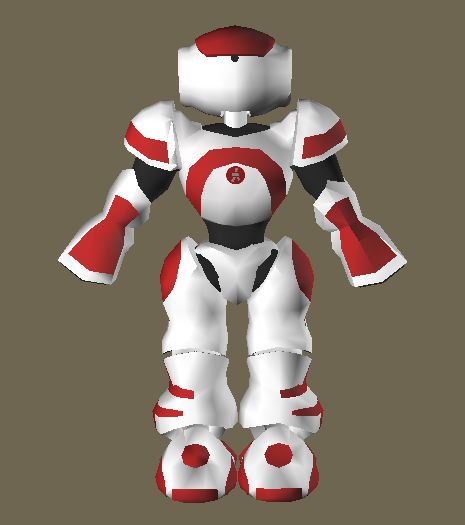
\includegraphics[height=0.28\columnwidth]{figs/NaoFront.png}&
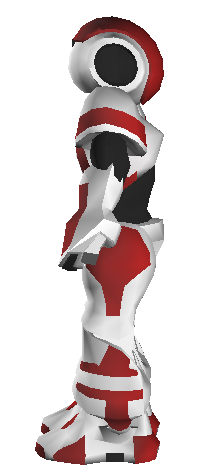
\includegraphics[height=0.28\columnwidth]{figs/NaoSide.png} &
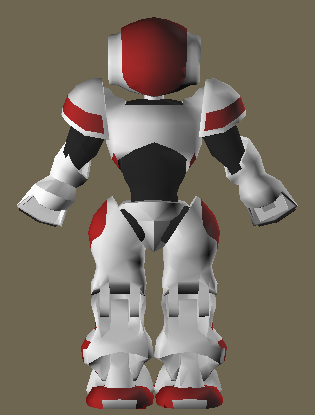
\includegraphics[height=0.28\columnwidth]{figs/NaoBack.png}
\end{tabular}}
\caption{Nao team markers. a) Front view. b) Side view. c) Back
view.} \label{fig:nao_markers}
\end{figure}

\subsection{Sponsorship/Team Logo Placement}
Teams may add a black and white logo to the upper part of the leg
(\cf Figure~\ref{fig:sponsor}). This logo must be at least 50\%
white by area.

\begin{figure}[b]
\centerline{\begin{tabular}{ll}
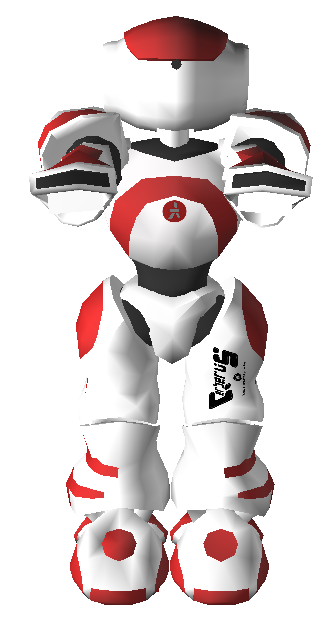
\includegraphics[height=0.35\columnwidth]{figs/RobotWithLogo.png}&
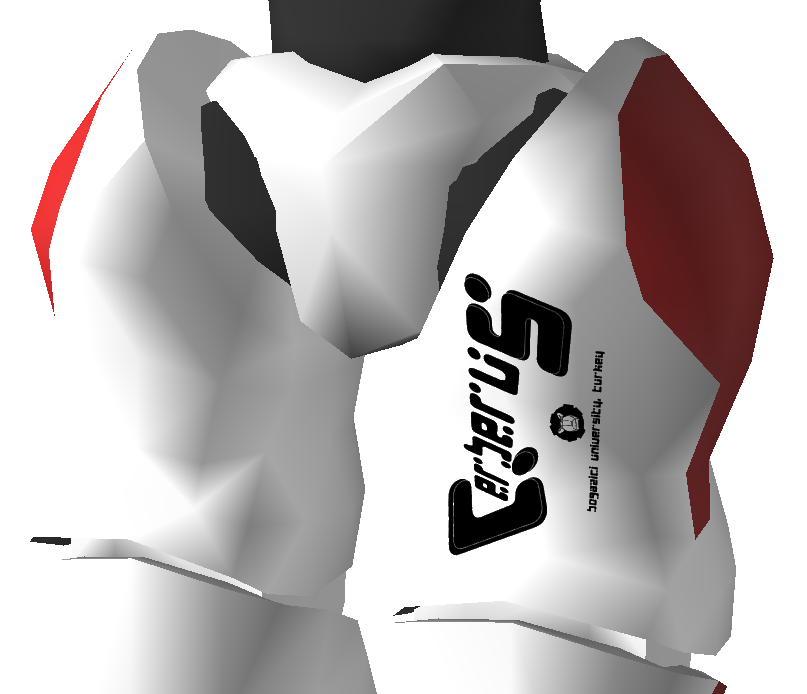
\includegraphics[height=0.35\columnwidth]{figs/sponsor.png}
\end{tabular}}
\caption{Example Sponsor/Team Logo placement.}
\label{fig:sponsor}
\end{figure}


\subsection{Communications}

The robots should play without human control.  Communication is
only allowed among robots on the field and between the robots and
the referee's controller.

\subsubsection{Acoustic Communications}

There are no restrictions on communication between the robots using
a microphone or a speaker.

\subsubsection{Wireless Communications}

The only wireless hardware allowed to be used by the teams are the
wireless network cards built into the Naos, and the access points
provided by the event organizers. All other wireless hardware must be
deactivated. A team may be disqualified if one of the team members
violates this rule. The MAC-addresses of all Naos participating in
the competition will be registered. Only these MAC-addresses can be
reached through the access points provided by the event organizers.
In addition, the access points will be secured by different SSIDs
and WEP-keys. Two of the access points will be connected to PCs
running GameController. A third access point is used for practise.
It is connected to a switch with one port for each team. Teams must
bring their own ethernet cables.

Each team will get a range of IP-addresses that can be used both for
their robots and their computers. The IP-addresses, channels, SSIDs,
and WEP-keys of the fields will be announced at the competition
site.

Teams can use a bandwidth of up to 500 Kbps of the wireless. This
includes any data transferred, namely the actual payload and any
protocol overhead created, \eg, by TCP, UDP, or the GameController.

Any form of wireless robot-to-robot communication is allowed, as
long as it uses the access points provided by the event organizers
(using the so-called ad-hoc mode is prohibited), it does not
conflict with TCP/IP or UDP, and the maximum bandwidth allowed for
each team is not exceeded. Each team will be assigned a range of 256
IP-addresses that can be used for direct robot-to-robot
communication. Each team will also be allocated a limited range of
UDP ports on which broadcast will be permitted.

The GameController will use UDP to connect to the robots. The source
distribution of the GameController provides the header file
\emph{RoboCupGameControlData.h} that defines all messages sent by
the GameController to the robots. They correspond to the \emph{robot
states} described in Section~\ref{sec:robot_states}.

The use of remote processing/sensing is prohibited.

\section{Game Process}
%procedures
\subsection{Structure of the Game}

\label{sec:game_struct}

A game consists of three parts, \ie the first half, a half-time
break, and the second half. Each half is 10 minutes. The clock stops
during stoppages of play\footnote{This may not be the case during
the preliminary games.} (such as kick-offs after goals). The extra
time over ten minutes total is referred to as ``lost time''.  The
half-time break is also ten minutes, during this time both teams may
change robots, change programs, or anything else that
can be done within the time allotted.  In the preliminaries a game
can finish in a draw as no penalty shoot-out will follow.
In the finals a game that ends in a draw will be followed by
a penalty shoot-out (see Section~\ref{sec:penalty_shoot-out}).

The teams will change the goal defended and color of the team
markers during the half-time break.

\begin{figure}[t]
\centerline{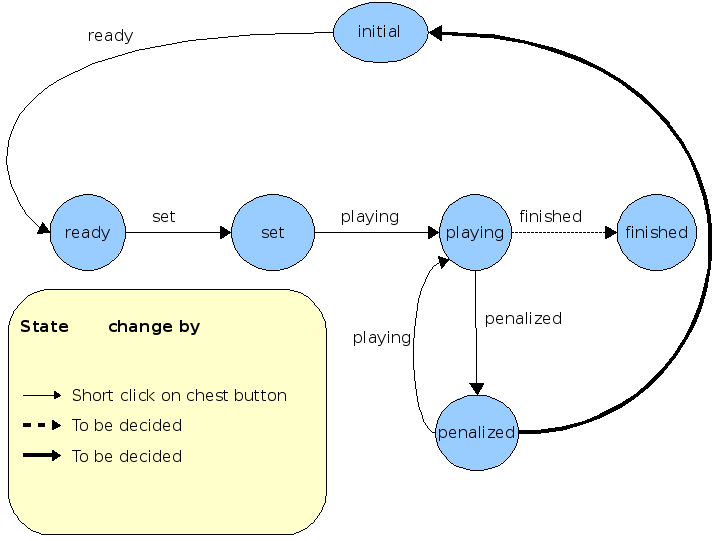
\includegraphics[width=0.9\columnwidth]{figs/states.png}}
\caption{Robot states.}
\label{fig:robot_states}
\end{figure}

\subsection{Robot States}
\label{sec:robot_states}

Robots can be in six different states (\cf
Figure~\ref{fig:robot_states}). If the wireless is available, these
states will be set by the GameController.  Teams must implement code to receive and correctly respond to wireless game controller packets, and also give indication of the game state, team color and the kickoff state.

%However, as the
%availability of the wireless cannot be guaranteed, it must also be
%possible to switch between the states manually. As the assistant
%referees handle the robots, the button interface must be the same
%for all teams. \textbf{Apparently, there is no simple solution for penalizing/unpenalizing but maybe we can use the bump sensors in the feet for init/ready/set/playing transitions. -Cetin}.


\begin{description}

\item[Initial.] After booting, the robots are in their \emph{initial} state. In this state, the button interface for manually setting the team color and whether the team has kick-off is active. The robots are not allowed moving in any fashion besides initially standing up. Pressing the left foot bump sensor will switch the team color while pressing the right foot bump sensor will switch the kickoff state. Shortly pressing the chest button will switch the robot to the \emph{ready} state.

%\textbf{Here, maybe we can use one bump sensor for transitions among states while using the other for enumerating blue-not-kick-off/blue-kick-off/red-not-kick-off/red-kick-off -Cetin}

%Pressing the bumper sensor on left foot will switch the robot to the \emph{ready} state.

\item[Ready.] In this state, the robots walk to their legal kick-off positions (\cf Section~\ref{sec:kick-off}). They remain in this state, until the head referee decides that there is no significant progress anymore (usually 45 seconds). Shortly pressing the chest button will switch the robot to the \emph{set} state.%By pressing the bump sensor on the left foot, it will be switched into the \emph{set} state.

Robots may be disentangled by the referees at the start of the Ready state.  After that, any robots which are close to each other (\cf Section~\ref{sec:player_pushing}) will be placed manually to the positions shown in Figure~\ref{fig:ko}.

\item[Set.] In this state, the robots stop and wait for kick-off (\cf Section~\ref{sec:kick-off}). If they are not at legal positions, they will be placed manually by the assistant referees to the positions shown in Figure~\ref{fig:ko}. They are allowed to move their heads before the game (re)starts but are not allowed moving their legs or locomote in any fashion. Shortly pressing the chest button will switch the robot to the \emph{playing} state.

%Pressing the bumper sensor on left foot will bring it to the \emph{ready} state, \eg for
%kick-off.

\item[Playing.] In the \emph{playing} state, the robots are playing soccer. Shortly pressing the chest button will switch the robot to the \emph{penalized} state.%\textbf{Penalizing/unpenalizing procedure is yet to be decided -Cetin}.
\item[Penalized.] A robot is in this state when it has been penalized. It is not allowed moving in any fashion, \ie also the head has to stop turning. Shortly pressing the chest button will switch the robot back to the \emph{playing} state.
\item[Finished.] This state is reached when a half is finished.
\end{description}

The team color should be displayed during the whole game. The
selection whether the robot's team has kick-off should be visible in
the states \emph{initial}, \emph{ready} and \emph{set}. Both
selections should also be visualized if the wireless is working. The current state of the robot should be displayed on the LED in torso and the LEDs on left and right foot should display the team color (blue/red) and whether the team has kickoff or not (white/off), respectively. The colors corresponding to the game states are:

\begin{itemize}
 \item Initial: Off
 \item Ready: Blue
 \item Set: Yellow
 \item Playing: Green
 \item Penalized: Red
 \item Finished: Off
\end{itemize}

\subsection{Goal}
A goal is achieved when the entire ball (not only the center of the
ball) goes over the goal-side edge of the goal line, \ie the ball
is completely inside the goal area\footnote{The goal line is part of
the field.}. The restart after the goal shall adopt the same
rules as the kick-off.

Note that a goal can never be awarded where the last contact of the ball with a robot was by the arm or hand (even if unintentional - see also Section~\ref{sec:hand_ball}) of an attacking robot. Should the ball enter the goal area where the last contact is accidental contact with the arm or hand of an attacking robot, the goal shall not count and a goal kick is awarded, that is, it shall count as if the ball is out by the attacking team (see Section \ref{sec:throw_in}).

\subsection{Applying Penalties}
See Section~\ref{sec:penalty_procedure}.

\subsection{Kick-off}
\label{sec:kick-off}

For kick-off, the robots listening to the wireless GameController
run through three states: \emph{ready},
\emph{set}, and \emph{playing}.  Robots not listening to the
GameController are simply penalized and manually placed for kick-off\footnote{
Note that robots being manually placed because they are not listening to the
GameController must still be placed in the restricted set of legal positions
for manually placed robots.  It is to a team's advantage to have their robots
listen to the GameController.}.

In the ready state, the robots should walk
to their legal kick-off positions. These positions are always
located inside their own side of the field. Only one field player
of the attacking team can walk to positions between the center line
and the middle of their side. He may put his leg(s) on the
center circle line, but no leg may be inside the circle line. The
other field players (one of attacking team, two of the defending team)
have to be located behind the middle of their side (none of their
legs are allowed to be in front of the middle line), and their feet must be outside the penalty area.
In contrast, the feet of the goal keeper must be \emph{inside}
the penalty area.

\textbf{If robots collide during the autonomous placement, the ``Player Pushing'' rules are applied, but
the penalty is manual placement by the assistant referees.}

The robots have a maximum of \KickOffAutoTime to reach their positions.
If all the robots have reached legal positions and have stopped, or
if \KickOffAutoTime has passed, the robots will be switched into the
\emph{set} state, in which they
must stop walking. Each robot that is not at a legal position at
this point in time will be placed manually by the assistant referees
to the positions as shown in Figure~\ref{fig:ko}. Robots
that are legally positioned will not be moved by the assistant
referees unless a manual position is requested by the team leader.

\begin{figure}[t]
\centerline{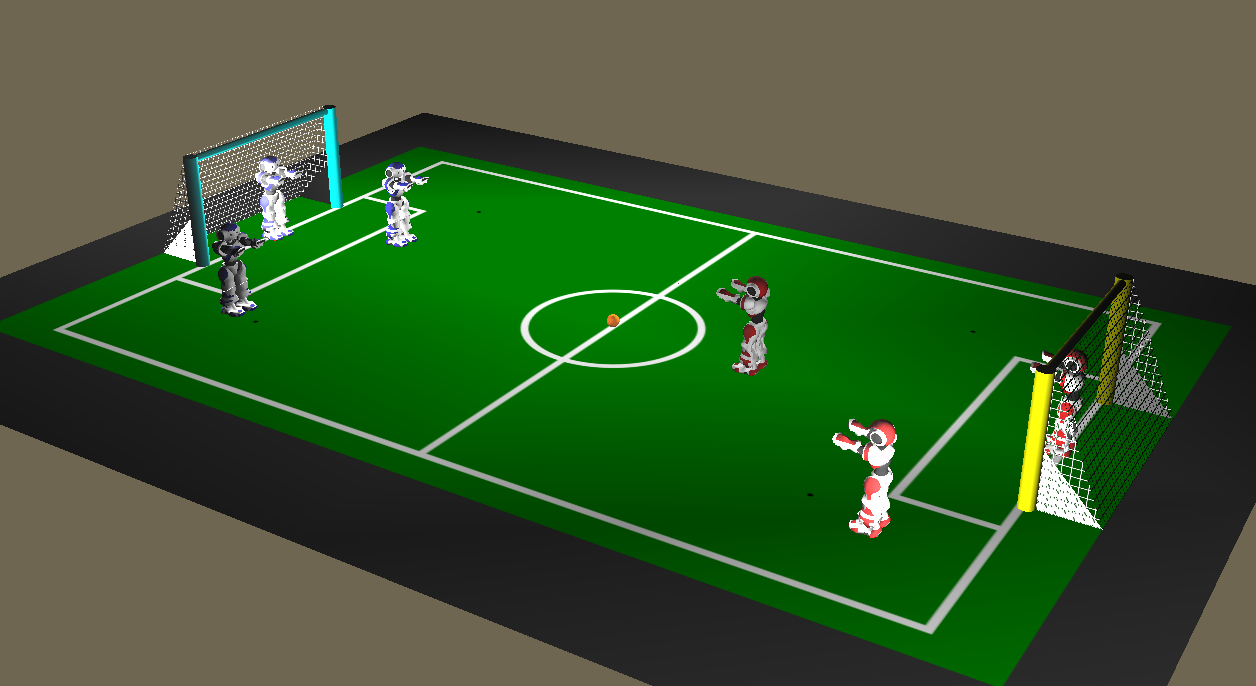
\includegraphics[width=\columnwidth]{figs/Kickoff3vs3}}
\caption{Manual setup for kick-off.}
\label{fig:ko}
\end{figure}

There are extra restrictions on the legal positions of manually
positioned robots. The kicking-off robot shall be 50cm
away from the center circle, while one robot of the team receiving the kick-off shall
be just in front of one corner of the penalty area. The other robots
shall be on the left and on the right of their own penalty area. As
autonomously placed robots are allowed to be much closer to the
ball, successful autonomous placement results in a significant
advantage over manual placement.

Just before the set state is called, the ball is placed on the
center point of the center circle by one of the referees.  If it
is moved by one of the robots before set is called it is replaced
by one of the referees.

After the head referee has signalled the kick-off, the robot's state
is switched to \emph{playing} (again either by the GameController or manually)
, in which they can actually play soccer.

Note that a goal can never be scored directly from a shot from the
kick-off. See Section~\ref{sec:kick-off_shot} for details.

If the assistant referees have misconfigured the robots (\eg they
set the wrong team color), the kick-off is repeated. In this case,
goals scored with at least one misconfigured robot on the field are
not counted. The time that was played with a wrong configuration is
counted as ``lost time'', \ie the half should be lengthened by it.
Note that the assistant referees are only responsible for setting team
color on kick-off.  Robots replaced after a request for pickup are
the responsibility of the team, %RHM 27/4/09
\emph{and should be handed to the referees or assistants in the `initial' state.}

The current GameController requires robots to know both their team number
and their robot number within the team.  It is each team's responsibility
to make sure this is correctly configured.  It is recommended that the
robot indicates its number within the team on bootup so that this can
be easily checked at the start of the game. %The example GameController
%object implements this functionality.

\subsection{Free Kick}
None.

\subsection{Penalty Kick}
\label{sec:penalty_kick}

A penalty kick is carried out with one attacking robot, playing as a red player, and one
opposing goal keeper, defending the blue goal. Other robots should be powered off and stay outside of the
field. Teams are allowed to switch to specially designed software
for a penalty kick. The attacker has 1 minute in which to score a
goal. If the ball leaves the playing area it is not replaced and
this penalty kick attempt is deemed unsuccessful.

Standard penalty kicks are taken against the opponent goal (\ie a
red robot will attack the blue goal). For a penalty shootout, see
Section~\ref{sec:penalty_shoot-out}.

The ball is placed on the penalty spot, at the end of the field closest to the goal being defended. The attacking robot is positioned at the center of the field, facing the ball. The goal keeper is placed with its feet on the
goal line and in the center of the goal.

Neither robot shall move their legs before the penalty kick starts. Movements of the
robot's head and arms are allowed as long as the robot does not
locomote. Technically, the robots are in the \emph{set} state when
waiting for the penalty kick to start. The robots are started by
switching to the \emph{playing} state.

The penalty
kick ends when the kicker scores the goal, the time expires or the
ball leaves the field. The time limit for the kicker is 1 minute
after the penalty kick starts. The ball must be in the goal within
this time limit in order to count as a goal.

The goal keeper is not allowed to touch the ball outside the penalty area (\ie one foot
outside) and the attacking robot is not allowed to touch the ball inside the penalty
area (\ie one foot inside the area). If the attacker touched the ball inside the
penalty area then the penalty shot is deemed unsuccessful. If the
goal keeper touches the ball outside the penalty area then a goal will be awarded to the
attacking team.

All the rules such as ``Ball Holding'', ``Pushing'' and
others are also applied during the penalty kick. The only exception
is the ``Illegal Defender'' rule, \ie the penalty shooter is allowed
to enter its own penalty area.

\subsection{Penalty Kick Shoot-out}
\label{sec:penalty_shoot-out}

A penalty kick shoot-out is used to determine the outcome of a tied
game when an outcome is required (for example, during quarter or semi finals).
The penalty kick shoot-out will initially consist of five
penalty shots \emph{per} team. At the conclusion of these shots the
team that has scored the most goals will be declared the winner. Note
that a winner can be declared before the conclusion of the penalty
shoot-out if a team can no longer win, for example, a team requires 3 goals
to win but only has 2 attempts remaining. If the two teams still
remain tied then a sudden death shoot-out will follow until a
definite winner is found.

The procedure for each attempt is the same as for the normal penalty
kick described in Section~\ref{sec:penalty_kick}. For the first five
attempts, the standard time limit of 1 minute is applied. If after five penalty kicks by each team
there is no result (that is, each team has scored the same number of goals), then the decision will be made by the following sudden death shoot-out procedure.

\subsubsection{Sudden Death Shoot-Out}

The time limit for sudden death penalty shots is two minutes.

These attempts will be timed (that is, for a goal scored, how long did it take to score the goal) and measured (that is, if a goal is not scored, what is the shortest distance between the ball and the goal line segment between the goal posts, achieved at any time during the penalty shot) by the referee. After these attempts, the game decision will be made as follows:
\begin{enumerate}
  \item {If only one team scores a goal, that team wins.}
  \item {If both teams score a goal, then if one team is timed to have scored at least 2 seconds faster than the other team, the faster team wins. Otherwise, the sudden death shoot-out is repeated.}
  \item {If neither team scores a goal, then if one team is measured to have moved the ball more than 50mm closer to the goal than the other team, the closer team wins. Otherwise, the sudden death shoot-out is repeated.}
  \item {If neither team has touched the ball during the shoot-out, the referee will toss a coin to decide the game.}
\end{enumerate}

\subsection{Throw-in}\label{sec:throw_in}

A ball is considered to have left the field when there is no part of the ball
over the outside of the boundary line  (\ie the line itself is in).
If the ball leaves the field it will be replaced on the field by an
assistant referee. There is \emph{no} stoppage in play.

If the ball goes over a side-line then the assistant referee will
replace the ball back on the field on the throw-in line on the same
side of the field as the ball went out of play.

The ball will be replaced on the throw-in line one metre (if possible)
back from the point it went out, where `back' is defined as being towards
the goal of the team that last touched the ball. Note that if the one metre placement would cause the ball to be placed
off the end of the throw-in line, then it should be placed at the end of the throw in line, and not beyond.

If the ball goes over an end-line then the assistant referee will
replace the ball back on the field according to the following rules:
\begin{itemize}
\item If the ball was last touched by the defensive team then the ball
  is replaced on the closest `corner kick' point. The `corner kick'
  points are located as indicated in Section \ref{sec:field_lines}.
\item If the ball was last touched by the offensive team then the ball
  is placed at the intersection of the halfway line and the throw in line on the side of the field the ball went
  out.
\end{itemize}

Balls are deemed to be out based on the team that last touched the
ball, irrespective of who actually kicked the ball.

\paragraph{Example 1.} The red goalie kicks the ball out the end of the
field to the right of the yellow goal.  The ball is placed on `corner kick' point
to the right of the yellow goal.

\paragraph{Example 2.} A blue robot kicks the ball out the end of the
field to the right of the yellow goal. The ball is placed on the intersection
of the right throw-in line and the halfway line.

\paragraph{Example 3.} A blue robot kicks the ball over the left
sideline 2 metres into the yellow half of the field. The ball is
replaced on the left throw-in line 1 metre into the yellow half of the field.

%\paragraph{Example 4.} The ball is kicked out over the end of the field.  The
%referees are not sure which robot was last to touch the ball.  The ball is
%replaced on the throw-in line 1 metre from the end of the field.

\paragraph{Example 4.} A blue robot kicks the ball but the ball
touches a red robot before leaving the field near the centre line.
The ball is regarded as out by red and therefore
is replaced on the throw-in line 1 metre closer to the yellow goal.

\subsection{Game Stuck}

The intention of the game stuck rules is to ensure some progress is made in the game, with minimal intervention from the referees.

\subsubsection{Local Game Stuck}

In the event of no substantial change in the game state for 30
seconds, the referee shall pick up the nearest robot to the ball and move the robot
to the half way line.  The referee does \emph{not} replace the ball.
If the ball is accidentally bumped when removing the robots, the ball should be replaced where
it was when the game stuck was called.  As a special exception, if
the goalie is involved in a game stuck situation while having one foot
in its own half (on half line or closer to goal), the goalie will
not be removed from the game stuck situation. Instead, the ball will be placed on the center point.

%\begin{figure}[htb]
%\centerline{
%\makebox[\columnwidth]{
%\hfill
%\includegraphics[height=5cm]{figs/local_game_stuck}\hspace{2cm}
%\includegraphics[height=5cm]{figs/local_game_stuck2}\hfill}}
%\caption{Local Game Stuck} \label{fig:stuck}
%\end{figure}

\subsubsection{Global Game Stuck}
If 
%RHM 27/4/09
\emph{following a local game stuck} no robot touches the ball for 30 seconds, the referee shall stop
the game and restart the game from the kick-off formation. The
kick-off will be awarded to the team defending the side of the field
the ball is on when the game stuck is called.

\subsection{Request for Pick-up}
Either team may request that one of their players be picked up only
for hardware dysfunction and software crashes at any point in the
game (called ``Request for Pick-up''). It is permitted to change
batteries, fix mechanical problems or, if necessary, reboot the
robots, but not to change or adjust their program. Any strategic
``Request for Pick-up'' is not allowed.  The head referee will
indicate when the robot is no longer affecting play and can be
removed from the field by an assistant referee.  The robot will be
replaced on the half way line after 30 seconds following the normal
replacement procedure used after the standard removal penalty (see
Section~\ref{sec:removal_penalty}).

If a robot has been rebooted and the wireless is not working, it is
the responsibility of the team members (not the assistant referees)
to configure its team color correctly.  The robot should be returned
to the assistant referees in the `Penalized' state so that the
assistant referees cannot accidentally change the robot's team color.

\subsection{Request for Timeout}

At any stoppage of play (after a goal, stuck game, before half,
etc.) either team may call a timeout.  Each team can call a maximum
of 1 timeout per game with a total time totalling no more than 5
minutes.  During this time, both teams may change robots, change
programs, or anything else that can be done within the time
allotted.  The timeout ends when the team that called the timeout
says they are finished, at which time they must be ready to play. At
this time the other team must either be ready to play or call a
timeout of its own.  The clock stops during timeouts, even during
the preliminaries.

After the completion of the timeout, the game resumes with a kick
off for the team which did not call the timeout.

If a team is not ready to play at the assigned time for a game, the
referee will call the timeout for that team. After the expiration
of such a timeout, if the team is still not ready to play then they
must either forfeit the game, or the referee shall start the game with
only one team on the field.   The team that wasn't ready can return
its robots to the field as per the rules for ``Request for Pick-up''.

%rankings
\subsection{Winner and Rankings}
The team which scored more goals than the other is the winner of the
match. If the two teams scored the same number of goals, the game
will be a draw. The draw will follow the same system defined in
Section~\ref{sec:game_struct}. Total (and final) standings will be
decided on points as follows (the points will be given based on the
result of each game):

\makebox[\columnwidth]{ \hfill Win = 3 pts\hfill Draw = 1 \hfill
Lose = 0 pts\hfill }

If a team's obtained points is the same as another team's after the
preliminary round is complete, the following evaluations will be
applied in order to qualify the finalists.

\begin{enumerate}
\item The points obtained
\item The average difference between goals for and goals against per game
\item The average goals for per game
\item Game result between the teams directly
\end{enumerate}


\subsection{Rules for Forfeiting}

If a team chooses to forfeit a match then the result will be 10-0 against the
team that forfeited. Teams may choose to forfeit games at any stage. Any game
with a final score differential greater than 10 points will be considered a forfeit.

\section{Forbidden Actions and Penalties}
\label{sec:forbidden_act}

The following actions are forbidden. In general, when a penalty
applies, the robot shall be replaced, not the ball.  For penalties
that are timed, the penalty time is considered to be over whenever
the game time stops (for goals, half-time, and game stuck).

\subsection{Locomotion Type}
\label{sec:locomotion_type}
Robots should clearly demonstrate bipedal walking similar to human walk. Other types of locomotion involving other parts than feet (crawling etc.) are strictly forbidden. It is duty of the head referee to decide whether a robot's locomotion is appropriate.

\subsection{Penalty procedure}
\label{sec:penalty_procedure}

When a robot commits a foul, the head referee shall call out the
infraction committed, the jersey color of the robot, and the jersey
number of the robot.  Each robot will be labeled with a jersey
number before the game.  The penalty for the infraction will be
applied immediately by an assistant referee.  The assistant referees
should perform the actual movement of the robots for the penalty so
that the head referee can continue focusing on the game.  The
operator of the GameController will send the appropriate signal to
the robots indicating the infraction committed.

\subsection{Standard Removal Penalty}
\label{sec:removal_penalty}

Unless otherwise stated (as for example in the case of the Goal Keeper, see Section \ref{sec:goal_keeper_standard_penalty}, all infractions in this league result in the removal of the
infringing robot from the field of play for 30 seconds, after which it will be returned to the field of play.
This process is called the standard removal penalty, and a detailed description of the process follows.

When the head
referee indicates a foul has been committed that results in the
standard removal penalty, the assistant referee closest to the robot
will remove the robot immediately from the field of play.  The robot
should be removed in such a way as to minimize the movement of the
other robots and the ball.  If the ball is inadvertently moved when
removing the robot, the ball should be replaced to the position it
was in when the robot was removed.

The operator of the GameController will send the appropriate signal
to the robot indicating the infraction committed.
If the wireless is
not working and the penalty is timed, the assistant referee handling
the robot will reset the robot into the \emph{penalized} state for
the duration of the penalty.
This may not be done if the penalty is not
timed, \ie it is a 0 seconds penalty. After a penalty is signalled
to the robot, it is not allowed to move in any fashion, such as being
in the \emph{initial} state. The removed robot will be placed
outside of the field facing away from the field of play.

The GameController will keep track of the time of the penalty. The
operator of the GameController will signal the assistant referees
when the penalty is over, so that one of them can put the robot back
on the field. The assistant referee will then place the robot on the
field on the halfway line as close to the sideline as possible.  The
robot should be pointed towards the opposite sideline.  The robot
should be placed on the side of the field furthest from the ball.
If there is another robot already in this position, the robot should
be replaced at a nearby location along the sideline facing towards
the opposite sideline.  If there are no practical locations nearby,
a location along one of the sidelines should be found that is away
from the ball (the robot should be set down facing the opposite
sideline).  When finding a nearby location, locations away from the
ball should be preferred.

When the robot is on the field again, the operator of the
GameController will send the \emph{playing} signal to it.
If the
wireless is not working, the assistant referee who placed the robot
back on the field has to bring it into the \emph{playing} state
again.

\subsubsection{Standard Penalty for the Goal Keeper}\label{sec:goal_keeper_standard_penalty}

In the case of infringements by a goal keeper, the standard removal penalty becomes a zero second removal. In this case, the robot will not be placed in the penalized state, and will be removed and immediately replaced at the sideline as in the standard replacement of a penalized robot.

\subsection{Manual Interaction by Team Members}

Manual interaction with the robots, either directly or via some
communications mechanism, is not permitted. Team members can only
touch one of their robots when an assistant referee hands it over to
them after a ``Request for Pick-up''.

\subsection{Kick-off Shot}
\label{sec:kick-off_shot}

A ``kick-off shot'' can never score a goal.  A ``kick-off shot'' is
a shot taken after a kick-off before the entire ball having left the
center circle, including the boundary line.  The ball must touch a
player from the kick-off team after leaving the center circle before
a goal can be scored by the team taking the kick-off.  If a kick-off
shot enters the goal (either directly or via contact with an
opposing robot), no goal will be scored and a kick-off will be
awarded to the defending team (as per Section~\ref{sec:kick-off}).

% \begin{figure}[t]
% \centerline{\includegraphics[height=0.3\columnwidth]{figs/parts}}
% \caption{Robot parts which are taken into account for ``Ball Holding''.}
% \label{fig:parts}
% \end{figure}

\subsection{Ball Holding}
\label{sec:ball_holding}

The goalie is allowed to hold the ball for up to 5 seconds as long
as it has one foot inside in its own penalty area.  In all other
cases, robots are allowed to hold the ball for up to 3 seconds.
Holding the ball for longer than this is ``Ball Holding'' and is not
allowed.

A robot which does not leave enough open space around the ball will
be penalized as ``Ball Holding'' if that situation continues more
than 3 seconds
% or if the robot moves the ball over 50cm while continuing to hold the ball.
The occupation of the ball is judged using the convex hull of the projection of the lower part of the robot's body (i.e. legs) onto the ground. ``Enough open space'' means that at least the half of the ball is not covered by the convex hull. It is not important whether the robot actually touches the ball.


\begin{figure}[t]
\centerline{\begin{tabular}{ll}
a) & b) \\
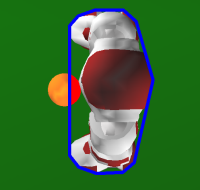
\includegraphics[scale=0.7]{figs/holding1} &
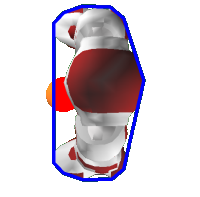
\includegraphics[scale=0.7]{figs/holding4}
\end{tabular}}

% \centerline{\begin{tabular}{ll}
% \\
% c) & d) \\
% 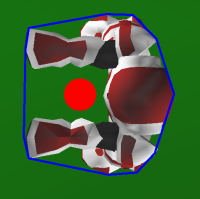
\includegraphics[scale=0.7]{figs/holding3}&
% 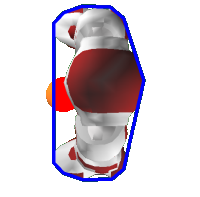
\includegraphics[scale=0.7]{figs/holding4}
% \end{tabular}}
\caption{Examples for ``Ball Holding''.  The orange circle is the ball, the blue polygon visualizes the convex hull of the robot's projection onto the ground and the red area shows the occupied portion of the ball. Situations a) is legal, whereas b) violates the rule.}
\label{fig:holding}
\end{figure}


Intentional continual holding is prohibited even if each individual
holding time does not continue for up to the time limit.  In general
robots should release the ball for approximately as long as they were
holding it to reset the clock.  Without a sufficient release,
the continual holding is regarded as a continuous hold from
the very beginning and the holding rule is strictly applied. The
violation of this rule will result in the standard removal
penalty (see Section~\ref{sec:removal_penalty} for details).  In
case of a violation by the goal keeper, the robot will be removed
for 0 seconds as per the standard removal penalty, \ie it will be
placed on the halfway line immediately (no need to be kept outside
of the field).  The ball should be removed from the possession of
the robot and placed where the foul occurred.  If the robot that
held the ball has moved the ball before the robot can be removed,
the ball shall be replaced where the foul occurred.

If a robot is transitioning from a hold into a dribble without holding,
then the robot should be careful to make a clear release of the ball
between the two movements.

It is not possible to score an offensive goal while holding the ball.  If the ball passes over the goal line while the robot is in holding position, then the ball is considered out
and the assistant referee shall replace it at the intersection of the
half line and the closer ``throw-in line''. However, it is still possible for a goal keeper to score a goal for the opposing team
while holding the ball.

\paragraph{Example.} A robot holds the ball and before the referees
can remove the robot, it shoots the ball into the goal.  The goal
will not be counted and the ball will be replaced where the robot
held the ball.

\subsection{Fallen or Inactive Robots}
\label{sec:fallenrobots}

If a robot falls during the game, it should start executing a getup action within 5 seconds. If it does not commence a get up action within 5 seconds, it will be removed as per the standard removal penalty. A robot which is unable to autonomously stand up within 20 seconds after a fall will be removed and subject to the standard penalty. The goal keeper, inside its own penalty area, is the only robot permitted to `dive' (that is deliberately fall in a way that might cause its torso, arms or hands) to intercept the ball. In all other cases, the robot should be programmed to attempt to remain upright - that is, supported by its feet.

A Robot that has ceased activity for 10seconds will be removed by the referees and subject to the standard removal penalty. A robot is active if it performs at least one of the following:
\begin{enumerate}
  \item {The robot walks in any direction, or turns.}
  \item {The robot searches for the ball, or is looking at the ball.}
\end{enumerate}

\paragraph{Note:} The intention of this rule is not to penalize robots simply for being stationary - provided they are not `asleep' and have not `crashed'.

%\subsection{Goalie Pushing}
%\label{sec:goalie_pushing}
%
%See \ref{sec:field_player_pushing}.

% When the goalie is in its own penalty area (one foot on or inside
% line), no attacker may be in contact with the goalie for more than 1
% second \textbf{or} be pushing the goalie indirectly through the
% ball for more than 1 second. If two attacking robots are
% simultaneously in contact with the goalie then the second attacking
% robot will be removed \textbf{immediately} and penalised for 30 seconds.
%
% Successive short pushes shall be counted as a single push even if each individual contact does not
% continue for a second.  A robot should obviously back off for
% at least as long as it pushed for the second clock to reset.
% When violating this rule the attacker will be removed for 30 seconds
% as per the standard removal penalty (see
% Section~\ref{sec:removal_penalty}).
%
% If a goal is scored by an action performed after a second of contact
% is over (or by a second robot that is touching the goalie), but before the
% robot can be removed, the ball and the robots involved in that
% action (the goalie, other robots, but not the penalized robot) shall
% be replaced where they were when the foul occurred.
%
% \paragraph{Example 1.} An attacker that has pushed the goalie shoots
% a goal after the violation but before it was removed. In that case,
% the goalie and the ball are replaced to the locations they were when
% the violation happened, and the goal is not counted.
%
% \paragraph{Example 2.} A second attacker scored a goal after the violation
% but before the pushing robot was removed. In that case, the goalie,
% the second attacker, and the ball are replaced to their original
% locations when the violation happened, and the goal is not counted.
% This is necessary, because the pushing robot prevented the goal
% keeper from defending its goal.
%
% \paragraph{Example 3.} An attacker that is currently pushing a
% goalie shoots a goal. If there has not yet been a second of contact
% between the attacker and the goalie, then the goal is allowed.

\subsection{Player Pushing}
\label{sec:player_pushing}

Except for the situations described below in Section \ref{sec:not_pushing}, no player should move in a direction that causes contact with another robot where, in the opinion of the referee, the contacting robot (or robots) should reasonably have been able to perceive the impeding robot, and avoid contact. Robots will be expected to be capable of looking in the direction they are moving, and perceiving nearby obstacles in the direction of their movement. Pushing with the arms is not permitted, however, a robot may use its arms for balance as part of its normal gait. Accidental contact with the hands or arms will not normally be penalized, unless it is in a position where the referee decides the robot should have been able to perceive likely contact.  Two robots may be penalized for pushing from the one incident, for example, if they collide front to front whilst both are moving.

\subsubsection{Situations where pushing does not apply}\label{sec:not_pushing}

A stationary robot cannot be penalized for pushing.

A robot will not be penalized for pushing whilst attempting to kick the ball, provided that the ball is close enough to the robot, that in the opinion of the referee the attempted kick could contact the ball.

The goal keeper, whilst in its own penalty area, and either moving to the ball or looking at the ball, will not be penalized for pushing.

A robot cannot be penalized for pushing if the contact is with a robot that is ruled to have deliberately moved to obstruct.

\subsubsection{Results of Player Pushing}

The standard removal penalty will apply for pushing. If the ball is moved as the result of pushing, then it will be replaced to where it was at the time of the infringement.

If a robot illegally pushes an opposing robot that is not pushing, and the collision causes the opposing robot to fall, the fallen robot will be picked up by one of the referees and replaced in an upright position at the point at which it fell.





%Any type of physical contact between robots is not allowed. In order to prevent physical contact, if two robots get within the falling distance of each other (50 cm), they will be moved 1m apart. If the encounter happens again in 3 seconds, the farther and/or the one which is not going to the ball will get a zero seconds penalty (it will be immediately placed on the halfway line at the opposite side of the field). Goalies cannot be called for violating the 50 cm rule as long as they stay in their own penalty area. Application of this rule to the teammates is left to the teams.  If a team wants to allow their robots to get close, this will be allowed. Further clarification on this rule will be discussed and finalized at RoboCup.
%
%
%%
%%Rick
%
%Any robot pushing another robot for more than 3 seconds will be
%removed from play for 30 seconds as per the standard removal penalty
%(see Section~\ref{sec:removal_penalty}).  The closest robot
%(including the goal keeper) to the ball on each team, if it is
%within 50cm of the ball, cannot be called for pushing.  If
%a robot is standing still it cannot be called for pushing.  If two
%moving robots are charging into each other then both robots are
%removed. The goalie cannot be called for pushing as long as it has
%at least two feet within its penalty area
%%Rick
%\emph{and is deemed to be active. Active means the goal keeper either:
%(i) is tracking the ball; (ii) has previously successfully seen the ball, and is now seeking to
%locate the ball}.
%
%\emph{A robot that: (a) has recently perceived the ball; (b) is within 50cm of the ball; (c) is active in moving towards the ball or positioning itself around the ball; and (d) is closer than any other robot, is said to have 'possession of the ball' (this should be clearly called by the referee, by a statement such as `Possession to Blue number 3'). Once a robot has possession of the ball, it cannot be called for pushing.}
%
%\emph{A robot loses possession of the ball when any of the following happens: (a) It becomes more than 50cm away from the ball (either by moving away from the ball, or by kicking the ball); (b) If in the opinion of the referee, it has lost direct perception of the ball for more than 15 seconds; or (c) An opposing robot that has previously been penalized for pushing against the same robot during the same possession of the ball, again approaches within 50 cm. In this latter case, the opposing robot gains possession of the ball, and the original robot is penalized for pushing.}
%
%
%
%\paragraph{Example 1.} A robot is going to the ball while a second robot approaches the ball from behind the first robot and the distance between two robots became smaller than 50cm. In that case the second robot will be removed.
%
%\paragraph{Example 2.} A robot is going to the ball while a second robot approaches the ball from the opposite direction of the first robot and the distance between two robots became smaller than 50cm. In that case the farthest robot will be removed.
%
%\paragraph{Example 3.} The ball is in front of a robot but the robot does not show interest in the ball while a second robot is approaching the ball and the distance between two robots became smaller than 50cm. In that case, the first robot will be removed.

\subsection{Playing with Arms/Hands}
\label{sec:hand_ball}
A field player or a goal keeper outside its own penalty box that intentionally touches the ball with its arms/hands in a manipulative manner (i.e. to stop the ball, to kick the ball etc.) will be subject to the standard removal penalty. In this case, the ball is to be replaced at the point where it contacted the arms/hands of the offending robot.


\subsection{Damage to the Field}

A robot that damages the field
will be removed from the field for the remainder
of the game. Similarly a robot that poses a threat to the
spectator's safety will also be removed. In such a case, a normal
penalty kick will be awarded to the opposing team (\cf
Section~\ref{sec:penalty_kick}).

\subsection{Leaving the Field}

A robot that leaves the \TotalWidth $\times$ \TotalLength carpeted area will be subject to the standard removal penalty (see
Section~\ref{sec:removal_penalty}).  A robot may leave the
4mx6m playing field, but must stay within the \TotalWidth $\times$ \TotalLength area.

A robot that chases the ball off the field, and then turns and moves
directly back onto the playing area when the ball is replaced on the
field, shall not be penalized.

\subsection{Illegal Defender}

Only the goalie can be within its team's penalty area. Having both
legs inside the penalty area is the definition of being in the
penalty area and that situation is not allowed for defending field
players.  When other defending robots enter the area, they will be
subject to the standard removal penalty (see
Section~\ref{sec:removal_penalty}).  This is called the ``Illegal
Defender Rule''.  This rule will be applied even if the goalie is
outside of the penalty area, but not if an operational defender is
pushed into the penalty area by an opponent.

If an illegal defender kicks an own goal, the goal is scored for the
opponent.  If there is any doubt about whether a goal should count
(e.g. The illegal defender infraction is called, but the robot scores
the own goal immediately afterwards, before it is removed) then the
decision shall be against the infringing robot.

\subsection{Obstruction}

 When a robot that is not heading for the ball is actively and
 intentionally blocking the way to the ball for a robot of the other
 team, this is an obstruction (\cf Figure~\ref{fig:obstruction}). The
 obstructing robot will be subject to the standard
 removal penalty (see Section~\ref{sec:removal_penalty}). A robot will not be penalized for pushing a robot that is penalized for obstruction (see Section~\ref{sec:player_pushing}).

 \paragraph{Example.} If a robot of one team, robot A, is heading for
 the ball, but a robot of the other team, robot B, is in its way without
 heading for the ball, this, by itself, is not an obstruction.  But,
 if robot A starts to move around robot B, and then robot B intentionally
 moves to block robot A again, this is an obstruction, even if the
 robots do not actually touch.

 Note:  The intent of the obstruction rule is to stop people
 implementing code that deliberately attempts to obstruct opponent
 robots.

 \begin{figure}[t]
 \centerline{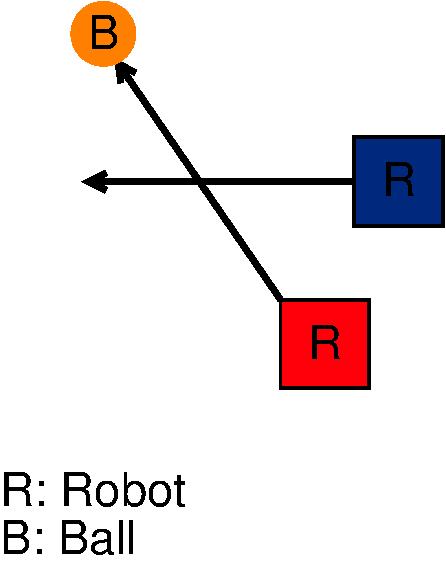
\includegraphics[height=5cm]{figs/obstruction}}
 \caption{Obstruction}\label{fig:obstruction}
 \end{figure}

\subsection{Jamming}

During the match any robot shall never jam the communication and the
sensor systems of the opponents:

\begin{description}

\item[Wireless communication.] Teams can use a bandwidth of up to 500 Kbps
of the wireless. This includes any data transferred, namely the actual
payload and any protocol overhead created, \eg, by TCP or UDP. If a team
uses more bandwidth over a couple of seconds in a game, it will be disqualified for that game.
Except for the wireless cards and the access points provided by the
organizers of the competition, nobody close to the field is allowed
using 2.4~GHz radio equipment (including cellular phones and/or
Bluetooth devices).
\item[Acoustic communication.] If acoustic communication is used by both
teams, they shall negotiate before the match
how they can reduce interference. If only one team uses acoustic
communication, the robots of the other team shall avoid producing
any sound. In addition, both the teams and the audience shall avoid
intentionally confusing the robots by producing similar sounds to
those used for communication.
\item[Visual perception.] To avoid confusing other robots, the robots are not allowed to switch LEDs to orange. In general, the use of flashlights is not allowed during the games.
\end{description}

\section{Judgement}

The referees are the only persons that are allowed inside the
playing area.

\subsection{Head Referee}

The head referee signals game starts, restarts, when a goal was
scored, the case of \emph{game stuck}, and penalties by a single
whistle. In general, the head referee first whistles and then
announces the reason for the whistle. The only exception is the case
of the kick-off, in which the reason for the whistle is obvious. The
whistle defines the point in time at which the decision is made. If
the head referee has to announce many decisions in short sequence,
he may skip whistling. For penalties, he announces the infraction
committed, the team color, and the jersey number of the robot, \eg
``illegal defender, blue number 3''. In case of a goal scored, local
or global game stuck, this is also announced verbally. By two
whistles, the head referee terminates the first half; by three
whistles he terminates the second half, \ie the whole game. The head
referee is also responsible for keeping the time of each half, \ie,
he or she stops the clock after a goal or game stuck, and continues
it at the kick-off\footnote{The clock may not be stopped during the
preliminaries.}. The head referee may choose to delegate this task
to the gamecontroller, it should be noted that the ultimate
responsibility for correct time keeping still remains with the head
referee.

In the penalty kick shoot-out, the head referee keeps the time.

Any decision of the head referee is valid. There is no discussion
about decisions during the game, neither between the assistant
referees and the head referee, nor between the audience or the teams
and the head referee.

\subsection{Assistant Referees}

The two assistant referees handle the robots. They start them if the
wireless is not working, they move them manually to legal kick-off
positions, they take them out when the robots are penalized, and
they put them in again. If a team requests picking up a robot, an
assistant referee will pick it up and give it to one of the team
members. An assistant referee will also put the robot back on the
field. In addition, the assistant referees can indicate violations
against the rules committed by robots to the head referee, so that
the head referee can decide whether to penalize a certain robot or
not. Assistant referees should only enter the field to execute a decision made by the main referee. They should not prevent robots from falling during the game.

\subsection{Operator of the GameController}

The operator of the GameController sits at a PC outside the playing
area. He or she will signal any change in the game state to the
robots via the wireless as they are announced by the head referee.
He or she will also inform the assistant referees when a timed
penalty is over and a robot has to be placed back on the field. The
operator may also be responsible for time keeping if the head
referee has delegated this task.

\subsection{Selection of the Referees}

At least in the preliminaries, the games will be refereed by members
of teams from a different Round-Robin group. Each team has to
referee a number of these games. For each of the games, it can
either provide the head referee and the operator of the
GameController, or the two assistant referees. These persons must
have good knowledge of the rules as applied in the tournament, and
the operator of the GameController must be experienced in using that
software. The persons should be selected among the more senior
members of a team, and preferably have prior experience with games
in the RoboCup Standard Platform (formerly Four Legged) league.

Referees for playoff games will need to be certified (\ie deemed fit to referee)
by at least half the teams in the playoffs. Unless they have no eligible referees,
each team in the playoffs shall supply at least one referee for the playoffs.
For a particular game, each of the teams playing shall be able to veto one
and only one eligible referee with no reason required.

\subsection{Referees During the Match}

The head referee and the assistant referees should wear black
clothing and black socks/shoes and avoid reserved colors for the
ball, the goals, and player markings in their clothing. They may
enter the field in particular situations, \eg, to remove a robot
when applying a penalty. They should avoid interfering with the
robots as much as possible.

\section{Questions/Comments}

Questions or comments on these rules should be mailed to
spl\_tech@tzi.de

\end{document}

